\chapter{Recherche}
\label{sec:recherche}


\section{A* Algorithmus}
Das Thema Wegfindung spielt in diesem Projekt eine wichtige Rolle. Der Computergegner soll einen Wegfindungs-Algorithmus benutzen, um den kürzesten Weg zum Ziel finden. Dabei soll die Wegfindung schnell und zuverlässig sein, auch wenn dynamisch ein oder mehrere Hindernisse auftauchen. In Kapitel \ref{sec:fundamentalsA*} wird die Funktionsweise des Algorithmus erläutert. An dieser Stelle soll deutlich werden warum sich in diesem Projekt für den A* Algorithmus entschieden wurde.

Zu den bekanntesten Algorithmen der Wegfindung gehören Dijkstra und A*. In Tabelle \ref{tbl:comparisonA*Dijkstra} werden die Vor- und Nachteile dieser Algorithmen gegenüber gestellt. Die Entscheidung für den A* Algorithmus ist aufgrund der Optimierung für die Suche mit nur einem Ziel. Das erhöht die Performanz, was bei einem Spiel zu einem besseren Spielfluss führen kann.


\begin{table}[H]
    \centering
    \resizebox{\textwidth}{!}{%
        \begin{tabular}{|l|p{5cm}|p{5cm}|}
            \hline
            \textbf{Algorithmus} & \textbf{Vorteile} & \textbf{Nachteile} \\ \hline
            Dijkstra & 
        \begin{minipage}{\linewidth}
            \vspace{0.1cm}
            \begin{itemize}
                \item Das Ziel muss nicht bekannt sein.
                \item Gut geeignet bei mehreren Zielen
            \end{itemize}
            \vspace{0.1cm}
        \end{minipage}         &
        \begin{minipage}{\linewidth}
            \vspace{0.1cm}
            \begin{itemize}
                \item Es wird der kürzeste Weg gefunden, bis dahin werden aber auch unnötige Pfade gegangen.
                \item Liefert fehlerhafte Ergebnisse bei negativen Kanten
            \end{itemize}
            \vspace{0.1cm}
        \end{minipage}                    \\ \hline
            A*		 &
          \begin{minipage}{\linewidth}
            \vspace{0.1cm}
            \begin{itemize}
                \item Verwendung einer Heuristik, um zielgerichtet zu suchen.
                \item Höhere Performanz durch zielgerichtete Suche.
                \item Er ist komplett, da er immer einen Weg findet, solange einer existiert
                \item Kann in einen anderen Path-Finding Algorithmus umgewandelt werden, indem man die Heuristik wechselt
            \end{itemize}
            \vspace{0.1cm}
        \end{minipage}            & 
          \begin{minipage}{\linewidth}
            \vspace{0.1cm}
            \begin{itemize}
                \item Nicht hilfreich wenn es mehrere Ziele gibt, da man nicht sagen kann welches das naheliegenste Ziel ist.
            \end{itemize}
            \vspace{0.1cm}
        \end{minipage}                    \\ \hline
        \end{tabular}%
    }
    \caption{Vergleich A* und Dijkstra }
    \label{tbl:comparisonA*Dijkstra}
\end{table}

\section{ImageTargets}
\label{sec:rec_imageTargets}
\begin{wrapfigure}{r}{0.2\textwidth}
	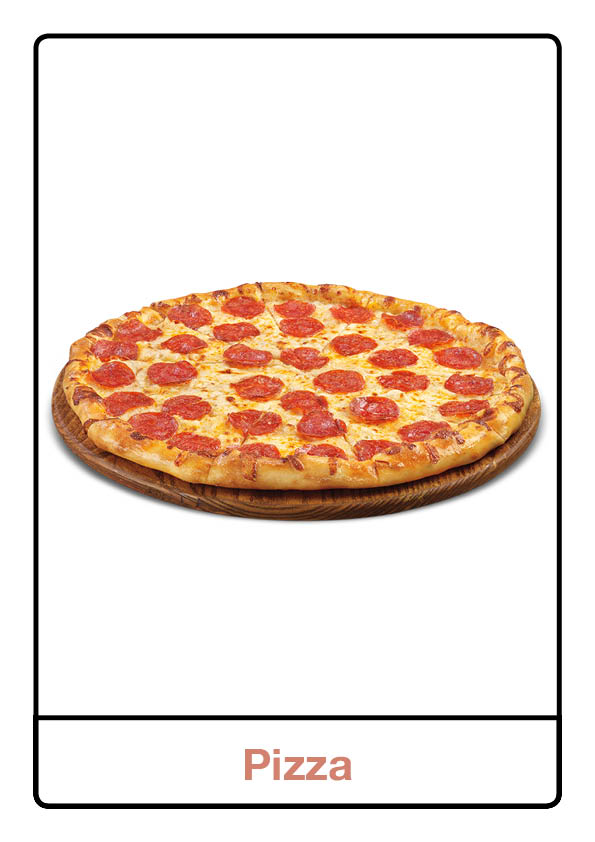
\includegraphics[width=3cm]{assets/exampleImageTarget.jpg}
	\caption{Beispiel ImageTarget}
	\label{fig:exampleImageTarget}
\end{wrapfigure}
ImageTargets sollen im Projekt RunnAR als Hindernisse wie auch als mögliches dynamisches Ziel für den Spieler dienen. Aus diesem Grund wurden vier unterschiedliche ImageTargets in die Vuforia Datenbank eingefügt, die dem Spieler als Hindernis dienen sollen. Wie im Kapitel \ref{sec:fund_imagetargets} \nameref{sec:fund_imagetargets} müssen die ImageTargets über möglichst viele eindeutige Merkmale verfügen. Die Vuforia Datenbank verfügt über eine Funktion zur Berechnung eines Rankings, anhand derer sich die ImageTarget Erkennungsqualität ablesen lässt. Nach erfolgreicher Recherche stellt sich heraus, dass Bilder mit einem weißen Hintergrund und einem eindeutigen Bild mit unterschiedlichen Merkmalen das höchstmögliche Maß an Wiedererkennungswert besitzt (siehe Abbildung: \ref{fig:exampleImageTarget}).

\todo{finde den Absatz scheiße. Weiß aber auch nicht was ich sonst dazu schreiben soll.}

\section{Objekterkennung}
Da die Objekterkennung einen großen Anteil des RunnAr Projekts ausmacht, wurde hierzu viel Recherche betrieben. Da die Objekte vom Benutzer in Echtzeit platziert und manipuliert werden können, wurde besonderes Augenmerk auf die Performanz der Implementierungsmöglichkeiten gerichtet.
\subsection{Tensorflow}
Tensorflow ist ein von Google entwickeltes Framework. Es wird oftmals in Programmen für maschinelles Lernen genutzt.  Implementiert ist es in Python und C++. Da Unity von Haus aus mit C Sharp Skripten arbeitet und keine alternative Sprache genutzt werden kann, muss für Unity das TensorFlowSharp Plugin genutzt werden. Dies stellt Wrapper zur Verfügung die den nativen C++ Code in C Sharp Code umwandeln. Auf Github finden sich einige Beispielprojekte, die den Fokus auf Objekterkennung setzen. Dies ermöglicht einen schnellen Einblick auf die Funktionalitäten von Tensorflow in Kombination mit Unity. Tensorflow ermöglicht es zwar durch trainierte Agenten eine große Variante an Objekten zu erkennen und zu klassifizieren, jedoch braucht dies seine Zeit. Die Kamera muss sich recht nah am Objekt befinden und Tensorflow verliert immer wieder den Fokus auf das Objekt. Zusätzlich ist die bounding Box, die sich um das Objekt dargestellt wird, recht grob. Bei diesem Ansatz fehlte für das Projekt also die Performanz und die Genauigkeit. Zusätzlich passte die Nähe die die Kamera zu dem Objekt haben musste nicht zu unserem Spielkonzept.

\subsection{OpenCv}
OpenCV ist eine freie Programmbibliothek zur Bildverarbeitung. Der Ansatz bei OpenCv wäre, dass Umrisse von auf dem Tisch platzierten Gegenständen erkennt werden sollten. Dies müsste jedoch auf einem hellen Untergrund geschehen, an dem sich die Objekte deutlich abheben. Der Vorteil gegenüber Tensorflow wäre hierbei, dass man keine trainierte Agenten bräuchte, die die Objekte zusätzlich klassifizieren würden. OpenCV hat jedoch den Nachteil, dass der Einsatz mit Unity kostenpflichtig ist. Die Kombination mit Unity ohne Kosten gestaltet sich als schwierig. Da Unity nur mit C Sharp Skripten arbeiten kann, müssten Wrapper erstellt werden, die die Kommunikation zu Unity ermöglichen würden. Fragwürdig wäre jedoch wie performant die Erkennung der Objekte mit OpenCv gewesen wäre.Viel Zeit und Aufwand hätten in die Entwicklung eines C++ Projekts mit OpenCv fließen müssen, bei der am Ende immer noch die Frage im Raum gewesen wäre, ob dies überhaupt flüssig in Unity laufen würde. Diesen Ansatz haben wir nach mehreren Tagen erfolgloser  Recherche und Implementierungsversuchen für ineffizient eingestuft. 

\subsection{Vuforia Object Recognition}
\label{sec:vufObjRec}
Vuforia verfügt nativ über Object Recognition. Hierbei müssen die Objekte, welche erkannt werden sollen, vorher durch eine kostenlose App für Android Geräte eingescannt werden. Hierfür kann man sich auf der Webseite von Vuforia eine Schablone ausdrucken, auf der man die zu scannenden Objekte platziert. Danach nutzt man die App und scannt die Objekte mit der Kamera auf dem mobilen Endgerät ein. Es wird virtuell ein Gitter um das platzierte Objekt dargestellt und die Bereiche die fertig gescannt wurden, werden grün markiert. Dies wiederholt man solange bis das Gitter komplett grün gefärbt ist.  Beim einscannen sollte man keine Objekte nehmen die zu klein sind, da diese recht lange brauchen um eingescannt zu werden. Zusätzlich ist die Erkennung kleiner Objekte nicht sehr effektiv, da Vuforia bei kleinen Objekte nicht ausreichend Vergleichspunkte hat um die Gegenstände zu erkennen. Die Performanz der eingescannten Objekte ist sehr gut, sodass die Einschränkung, dass nur eingescannte Objekte erkennt werden können, in Kauf genommen wurde. Auch die Erkennung über weite Entfernungen ist gegeben. Nach dem Einscannen, können diese in eine Datenbank importiert und problemlos in Unity eingebunden werden. Mehr zu diesem Thema im Kapitel Umsetzung.
